\scanpage{120}
% Writing on ruled music paper. Turn the archive image through 180 degrees.
% archive sheet number: 121
\figure{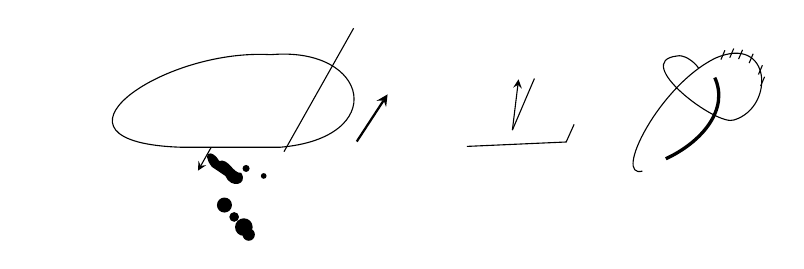
\begin{tikzpicture}[scale=.56,>=stealth]
\draw (0,0) .. controls (-3.5,.1) and (-.5,2.25) .. (2,2.1) .. controls (4.25,2.3) and (4.7,.2) .. (2.2,0) -- cycle;
\draw[->,thick] (3.95,.13)--(4.65,1.2); \draw[->] (.65,0)--(.35,-.53);
\draw (2.3,-.1)--(3.88,2.7);
\draw (6.45,.02)--(8.7,.12)--(8.88,.52); \draw[->] (7.48,.39)--(7.62,1.54); \draw (7.48,.39)--(7.98,1.56);
\draw (10.43,-.54).. controls (9.75,-.72) and (10.8,1.39)..(12.08,2.02)..controls(13.36,2.58)and(13.44,.91)..(12.51,.62)..controls(12.12,.46)and(10.16,1.95)..(11.21,2.07)..controls(11.36,2.11)and(11.59,1.96)..(11.7,1.8);
\draw[very thick] (10.96,-.26)..controls(11.78,.12)and(12.4,.86)..(12.07,1.58);
\foreach \x/\y in {12.25/2.08,12.45/2.12,12.65/2.09,12.89/2.0,13.1/1.74,13.15/1.48}{\draw (\x-.04,\y-.09)--(\x+.05,\y+.12);}
\fill (.66,-.44) ..controls(.4,-.09)and(.69,-.04)..(.83,-.31)..controls(1.05,-.24)and(1.14,-.6)..(1.33,-.58)..controls(1.5,-.85)and(1.09,-.95)..(.97,-.65)--cycle;
\foreach \x/\y/\r in {1.44/-.48/.08,1.84/-.65/.065,.95/-1.31/.17,1.17/-1.58/.11,1.39/-1.81/.2,1.5/-1.98/.14}{\fill (\x,\y) circle (\r);}
\end{tikzpicture}}
\[
\deleted{\unsure{P|p}}\quad \Gamma\longrightarrow S^1
\]
\[
 S^2\times S^2-\mathrm{diag}\qquad
 {\displaystyle S^2\times S^2/\mathord{\pm}1}\ \deleted{\unsure{-|/}}\Delta
\]
\diagram{\begin{tikzcd}[ampersand replacement=\&,column sep=.55em]
 {}\&{}\&\pi_1(S^1)=\mathbb Z\arrow[d,"2"']\\
 {}\&{\unsure{\mathbb C|C}}^{*}\arrow[d]\&\pi_1(C^{\unsure{*|1}})=\mathbb Z\arrow[d]\\
 {\deleted{S^2\times S^2-\mathrm{diag}-\unsure{\mathrm{antidiag}|\mathrm{antid}}} =}\&\unsure{\mathbb P|P}\arrow[d]\&\pi_1(\unsure{\mathbb P|P})\arrow[d]\\
 S^1\arrow[r]\&S^2\&\pi_1(S^2)=0
\end{tikzcd}}
\[
 (x,y)\qquad\begin{array}{l}\deleted{\unsure{y}=x}\\ y=-x\end{array}
\]
\figure{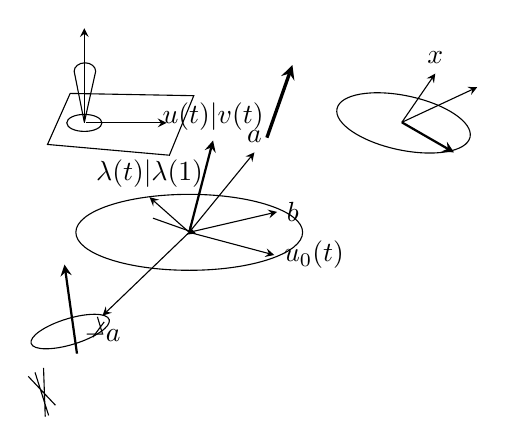
\begin{tikzpicture}[scale=.72,>=stealth]
\draw (-2.1,1.55)--(-2.5,.65)--(-.35,.46)--(.08,1.51)--cycle;
\draw (-1.85,1.03) ellipse (.31 and .15); \draw (-1.85,1.04)--(-2.03,1.94) arc[start angle=180,end angle=0,x radius=.19,y radius=.15]--(-1.85,1.04);
\draw[->] (-1.85,1.03)--(-1.85,2.7);\draw[->](-1.82,1.03)--(-.4,1.03);
\draw (0,-.9) ellipse (2 and .67);
\draw[->] (0,-.9)--(-.7,-.28) node[above]{$\unsure{\lambda(t)|\lambda(1)}$};
\draw[->,thick] (0,-.9)--(.42,.72) node[above]{$\unsure{u(t)|v(t)}$};
\draw[->] (0,-.9)--(1.15,.51) node[above]{$a$};
\draw[->] (0,-.9)--(1.55,-.54) node[right]{$b$};
\draw[->] (0,-.9)--(1.5,-1.3) node[right]{$u_0(t)$};
\draw[->] (0,-.9)--(-1.53,-2.37) node[below]{$-a$};
\draw[->,very thick] (1.37,.77)--(1.82,2.05); \draw[->] (-.64,-.65)--(.12,-.92);
\draw (-2.1,-2.65) ellipse[x radius=.72,y radius=.23,rotate=17]; \draw[->,thick](-1.98,-3.04)--(-2.2,-1.47);
\draw (-1.5,-2.48)--(-1.7,-2.75) (-1.62,-2.39)--(-1.53,-2.69);
\draw (-2.72,-3.37)--(-2.48,-4.13) (-2.84,-3.44)--(-2.36,-3.95) (-2.57,-3.29)--(-2.54,-4.15);
\draw (3.78,1.03) ellipse[x radius=1.2,y radius=.48,rotate=-12];
\draw[->] (3.75,1.04)--(4.34,1.9)node[above]{$x$};
\draw[->] (3.75,1.04)--(5.08,1.66);
\draw[->,thick] (3.75,1.04)--(4.67,.51);
\end{tikzpicture}}
\[
 \unsure{\theta|\Theta}(t): S^1\longrightarrow S^2 \qquad
 \deleted{{\unsure{P|p|\mathbb P}}^1\times P^1-P^1}
\]
\diagram{\begin{tikzcd}[ampersand replacement=\&,row sep=small]
 {}\&{}\& L\\
 X\times\&E\arrow[ur]\arrow[dr]\&{}\\
 F\arrow[ur,dash]\arrow[rr,"\sim"']\&{}\& L'
\end{tikzcd}}
\[
 \underline{1\text{-}\mathrm{hom}}\,(\unsure{h|u|L},F)\qquad E\simeq L\oplus L'
 \qquad \boxed{p^2=p\quad\mathrm{Tr}\,p=1}
\]
\[
 0\longrightarrow F\longrightarrow E_p\longrightarrow\underline{\mathcal O}(1)\longrightarrow0
\]
\[
 F\oplus\mathcal O(1)\simeq \unsure{\mathcal O|0}\qquad
 F\simeq\mathcal O(-1)\qquad \underline{\mathcal O}(-2)
\]
\figure{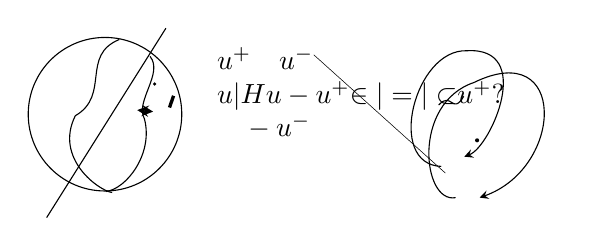
\begin{tikzpicture}[scale=.65,>=stealth]
\draw (0,0) circle (1.5); \draw (.28,1.46) .. controls(-.48,1.15)and(.11,.37)..(-.58,-.03)..controls(-1,-.87)and(-.11,-1.5)..(.14,-1.53);
\draw (.88,1.13)..controls(1.15,.8)and(.58,.25)..(.77,-.09)..controls(.95,-.77)and(.42,-1.46)..(.02,-1.51);
\draw[<->,thick] (.63,.08)--(.94,.05); \fill (.97,.59) circle (.035); \draw[very thick] (1.26,.13)--(1.34,.36);
\draw (-1.14,-2.02)--(1.19,1.68);
\node[anchor=west,align=left] at (2,.41){$u^+\quad u^-$\\$\deleted{\unsure{u|H}}u-u^+\unsure{\in|=|\subset}u^+?$\\$\phantom{u}\ -u^-$};
\draw[very thin] (4.08,1.16)--(6.65,-1.15);
\draw[->] (6.57,-1.02)..controls(5.48,-.98)and(6.05,1.28)..(7.07,1.24)..controls(8.4,1.32)and(7.54,-.63)..(7.02,-.83);
\draw[->] (6.85,-1.63)..controls(6.2,-1.75)and(5.99,.21)..(7.21,.62)..controls(9.04,1.51)and(8.97,-1.04)..(7.32,-1.63);
\fill (7.27,-.51) circle (.04);
\draw (6.52,.18) .. controls (6.78,.46)and(6.78,-.03).. (7.01,.35);
\end{tikzpicture}}
\figure{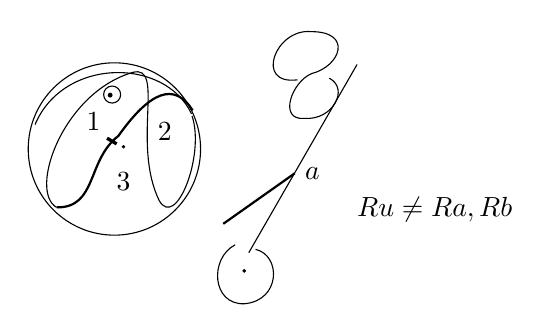
\begin{tikzpicture}[scale=.72,>=stealth]
\draw (0,0) circle (1.52); \draw (-1.4,.43)..controls(-.9,1.62)and(.89,1.62)..(1.36,.62);
\draw (-1.02,-1.03)..controls(-1.52,-.74)and(-.91,.99)..(.32,1.35)..controls(.9,1.51)and(.3,.1)..(.79,-.91)..controls(1.09,-1.43)and(1.6,-.1)..(1.37,.58);
\draw[thick](-1.02,-1.03)..controls(-.3,-1.04)and(-.49,-.2)..(.07,.23)..controls(.63,1.02)and(1.06,1.19)..(1.38,.68);
\draw (-.04,.96) circle(.15); \fill (-.075,.95) circle(.043); \draw[very thick](-.13,.19)--(.04,.09); \fill(.16,.04)circle(.034);
\node at(-.37,.49){$1$};\node at(.89,.31){$2$};\node at(.16,-.58){$3$};
\draw (3.23,1.22)..controls(2.46,1.12)and(2.84,2.13)..(3.47,2.07)..controls(4.21,2.07)and(3.99,1.46)..(3.48,1.33)..controls(3.13,1.19)and(2.88,.5)..(3.35,.54)..controls(3.85,.5)and(4.15,1.06)..(3.79,1.25);
\draw[thick] (1.92,-1.32)--(3.18,-.43)node[right]{$a$};
\draw (2.13,-1.69)..controls(1.67,-1.93)and(1.72,-2.75)..(2.29,-2.73)..controls(2.93,-2.68)and(2.95,-1.88)..(2.49,-1.77);
\fill (2.29,-2.15) circle(.035); \draw[thin] (2.37,-1.83)--(4.28,1.49);
\node at(5.65,-1.07){$\mathbb R u\ne\mathbb R a,\mathbb R b$};
\end{tikzpicture}}
% crop-candidate: scan 120
